\section{Spektren}
	\subsection{Spektraldarstellung}
		\begin{minipage}[t]{0.5\textwidth}
			%\scalebox{0.8}{\begin{tikzpicture}
	%axis
	\begin{scope} [decoration={border, segment length=1cm, amplitude=1mm, angle=90}]
		\draw[postaction={decorate, draw}] (-5, 0) -- (5.1, 0);
		\draw[postaction={decorate, draw}] (0, 0) -- (0, 5.1); 
	\end{scope}
	
	\def\lzero{(-5, 1) cos (-2.5, 1.5) sin (0,2) cos (2.5, 1.5) sin (5, 1)};
	\fill[cyan, opacity=0.2] \lzero;
	\draw[cyan!75!black] \lzero node[right, black] {$\Psi_0(x)$};
	
	\def\lone{(-5, 2.5) cos (-3.33, 2.25) sin (-1.66, 2) cos (0, 2.5) sin (1.66, 3) cos (3.33, 2.75) sin (5, 2.5)}
	\fill[red, opacity=0.2] \lone;
	\draw[red!75!black] \lone node[right, black] {$\Psi_1(x)$};
	
	\def\ltwo{(-5, 4) cos (-3.75, 4.25) sin (-2.5, 4.5) cos (-1.25, 4) sin (0, 3.5) cos (1.25, 4) sin (2.5, 4.5) cos (3.75, 4.25) sin (5, 4)}
	\fill[green, opacity=0.2] \ltwo;
	\draw[green!75!black] \ltwo node[right, black] {$\Psi_2(x)$};
	
	\draw (0, 0) parabola (5, 5);
	\draw (0, 0) parabola (-5, 5);
	
	\draw[latex-latex, red] (-5, -1.5) -- (5, -1.5);
	\node[above, red] at (0, -1.5) {$T = \dfrac{2 \pi}{\omega_f}$ von $f$};
	
	\draw[dashed, red] (-5, -1.5) -- (-5, 5);
	\draw[dashed, red] (5, -1.5) -- (5, 5);
\end{tikzpicture}}
			\textbf{Spektrum:} Fourierkoeffizienten einer Funktion.
		\end{minipage}
		\begin{minipage}[t]{0.5\textwidth}
			Fourierreihe des abgebildeten Beispiels:\\[3pt]
			$f(t) = \sum\limits_{k=1}^{\infty} \dfrac{1}{2k - 1} \cdot \sin((2k - 1) \cdot t)$
		\end{minipage}

	\subsection{(1) Kosinus- und Sinusamplitudendiagramm}
		\begin{minipage}[]{0.5\textwidth}
			\begin{tabular}{|l|l|}
				\hline
				\textbf{Kosinus-Amplituden} & \textbf{Sinus-Amplituden}\\[3pt]
				\hline
				\scalebox{0.45}{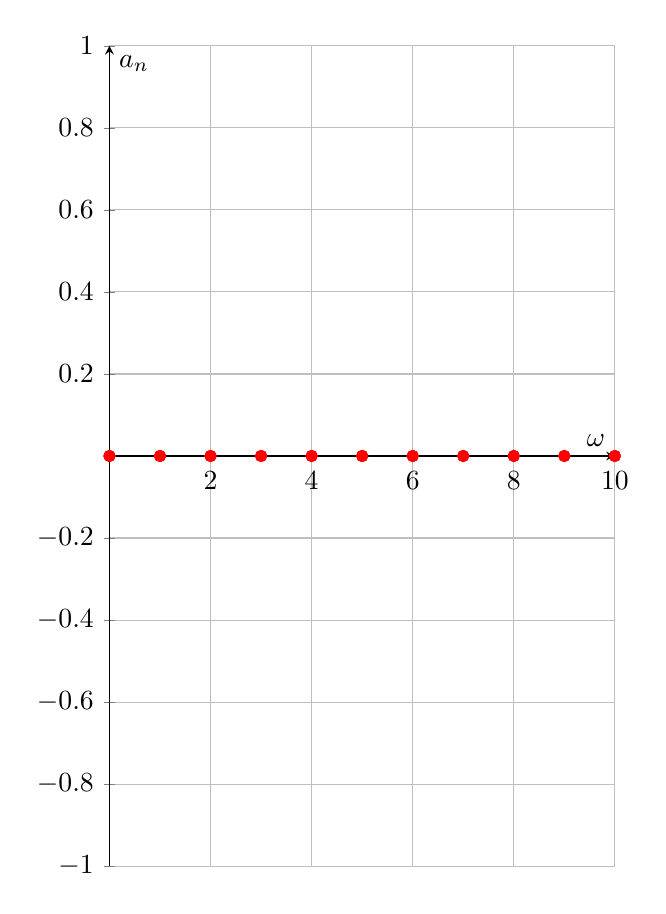
\begin{tikzpicture}
	\begin{axis}[axis lines=middle, grid=both, height=12cm, width=8cm, xmin=0, xmax=10, ymin=-1, ymax=1, xlabel = $\omega$, ylabel = $\operatorname{a_n}$]
		\foreach \x in {0,...,10}
		{ \addplot[mark=*, red] coordinates { (\x, 0) (\x, 0) }; }
	\end{axis}
\end{tikzpicture}} & \scalebox{0.45}{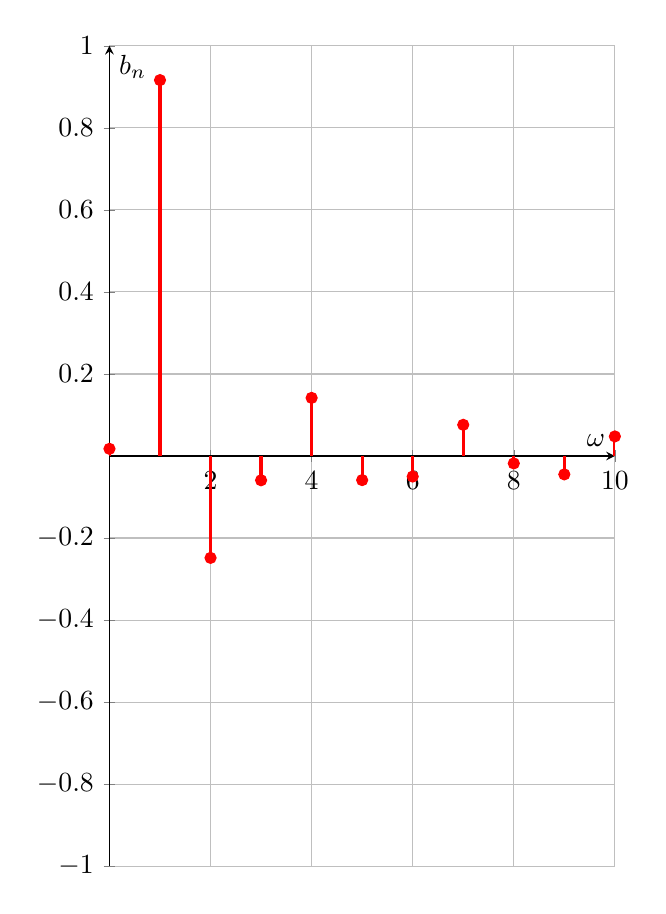
\begin{tikzpicture}
	\begin{axis}[axis lines=middle, grid=both, height=12cm, width=8cm, xmin=0, xmax=10, ymin=-1, ymax=1, xlabel = $\omega$, ylabel = $b_n$]
		\foreach \x in {0,...,10}{
			\addplot[mark=none, red, very thick] coordinates { (\x, 0) ({\x}, {1/(2 * \x - 1) * sin(2 * deg(\x) - 1)}) };
			\addplot[only marks, red] coordinates{ (\x, {1/(2 * \x - 1) * sin(2 * deg(\x) - 1)}) };
		}
	\end{axis}
\end{tikzpicture}}\\[3pt]
				\hline
			\end{tabular}
		\end{minipage}
		\begin{minipage}[]{0.5\textwidth}
			\textbf{Werte der reelen Fourierkoeffizienten $a_n$ und $b_n$ werden als ''Säulen'' dargestellt.}\\[3pt]
			Reelle Fourierkoeffizienten $(a_n, b_n)$ können direkt abgelesen werden.\\[3pt]
			\fbox{$a_n = A_n \cdot \cos(\varphi_n) = 2 \cdot \operatorname{Re}(c_n)$}\\[3pt]
			\fbox{$b_n = -A_n \cdot \sin(\varphi_n) = A_n \sin(-\varphi_n) = -2 \cdot \operatorname{Re}(c_n)$}\\[3pt]
			\textbf{Nachteil:} Diagramme sind vom Ort des Nullpunktes auf der Zeitachse abhängig.\\[3pt]
		\end{minipage}
	
	\subsection{(2) Einseitiges Amplituden-/Phasendiagramm}
		\begin{minipage}[]{0.5\textwidth}
			\begin{tabular}{|l|l|}
				\hline
				\textbf{Amplituden} & \textbf{Phasen}\\[3pt]
				\hline
				\scalebox{0.45}{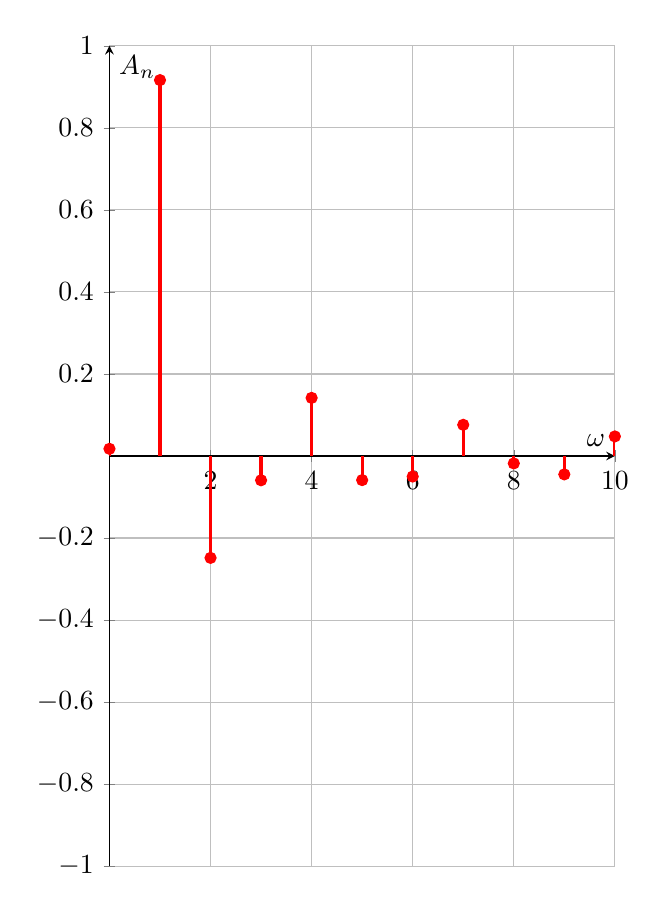
\begin{tikzpicture}
	\begin{axis}[axis lines=middle, grid=both, height=12cm, width=8cm, xmin=0, xmax=10, ymin=-1, ymax=1, xlabel = $\omega$, ylabel = $A_n$]
		\foreach \x in {0,...,10}{
			\addplot[mark=none, red, very thick] coordinates { (\x, 0) ({\x}, {1/(2 * \x - 1) * sin(2 * deg(\x) - 1)}) };
			\addplot[only marks, red] coordinates{ (\x, {1/(2 * \x - 1) * sin(2 * deg(\x) - 1)}) };
		}
	\end{axis}
\end{tikzpicture}} & \scalebox{0.45}{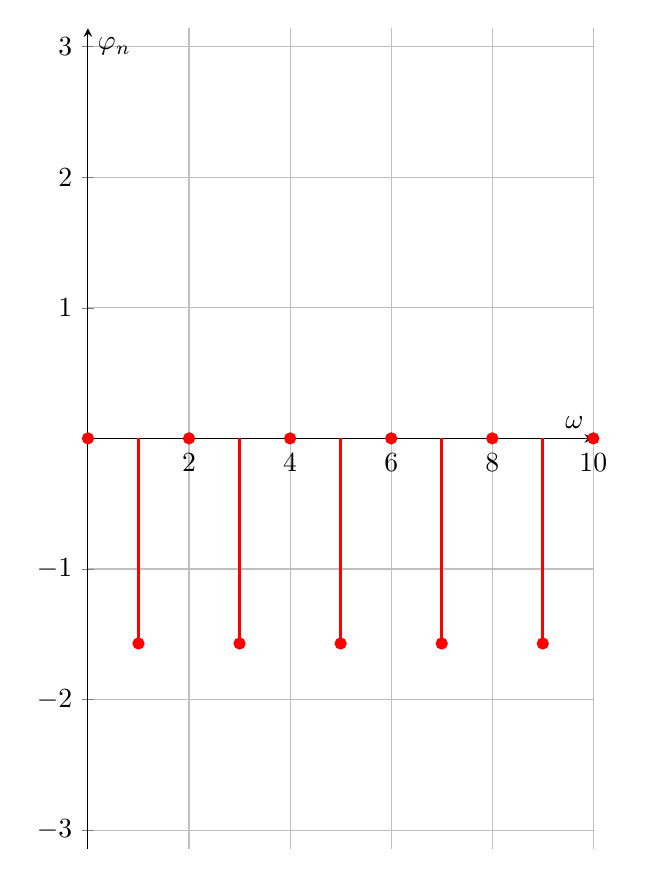
\begin{tikzpicture}
	\begin{axis}[axis lines=middle, grid=both, height=12cm, width=8cm, xmin=0, xmax=10, ymin=-pi, ymax=pi, xlabel = $\omega$, ylabel = $\varphi_n$]
		\foreach \x in {0,...,5}{
			\addplot[mark=none, red, very thick] coordinates { ({\x * 2 - 1}, 0) ({\x * 2 - 1}, {-pi/2}) };
			\addplot[only marks, red] coordinates{ ({\x * 2 - 1}, {-pi/2}) };
			\addplot[only marks, red] coordinates{ ({\x * 2}, {0}) };
		}
	\end{axis}
\end{tikzpicture}}\\[3pt]
				\hline
			\end{tabular}
		\end{minipage}
		\begin{minipage}[]{0.5\textwidth}
			\textbf{Gleichfrequente Schwingungen werden zu phasenverschobenen
				Kosinusschwingungen zusammengefasst: $a_n \cdot \cos(n \omega_f t) + b_n \cdot \sin(n \omega_f t) = A_n \cdot \cos(n \omega_f t + \varphi_n)$}\\[3pt]
			\fbox{$\varphi_n = \arg(a_n - \mathrm{j} b_n) = \arctan(-\dfrac{b_n}{a_n}) \text{ oder } \varphi_n = \arg(c_n)$}\\[3pt]
			\fbox{$A_n = |a_n - \mathrm{j} b_n| = \sqrt{a_n^2 + b_n^2} \text{ oder } A_n = 2 \cdot |c_n|$}\\[3pt]
			\textbf{Spezialfall: $n = 0$}\\[3pt]
			\fbox{$A_0 = |\dfrac{a_0}{2}|$} \fbox{$\varphi_0 = \left\lbrace 
				\begin{array}{ll}
					0\text{,} & a_0 \geq 0\\[3pt]
					\pi\text{,} & a_0 < 0\\[3pt]
				\end{array}
				\right. $}
		\end{minipage}\\[3pt]
	
	\subsection{(3) Zweiseitiges Amplituden-/Phasendiagramm (komplexes Spektrum)}
		\begin{minipage}[]{0.5\textwidth}
			\begin{tabular}{|l|l|}
				\hline
				\textbf{Amplituden (I)} & \textbf{Phasen (II)}\\[3pt]
				\hline
				\scalebox{0.55}{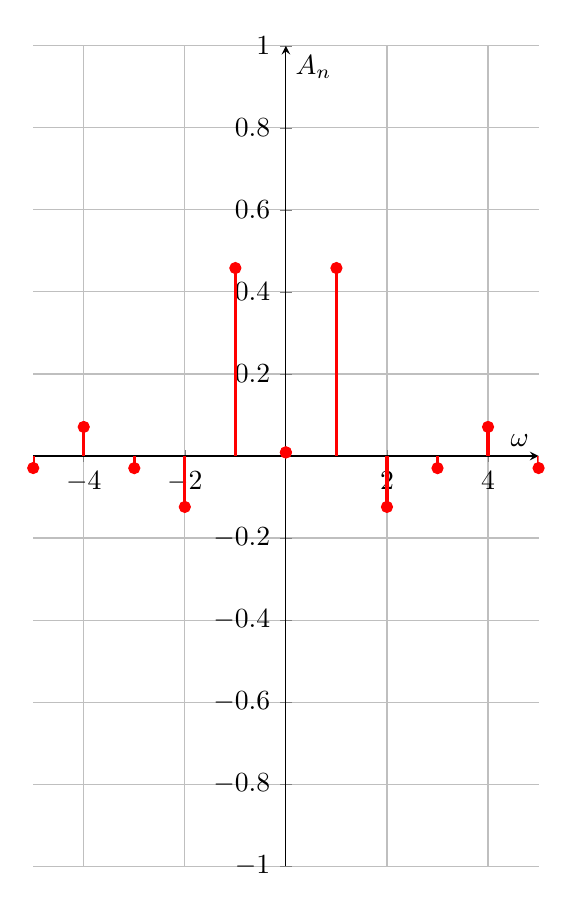
\begin{tikzpicture}
	\begin{axis}[axis lines=middle, grid=both, height=12cm, width=8cm, xmin=-5, xmax=5, ymin=-1, ymax=1, xlabel = $\omega$, ylabel = $A_n$]
		\foreach \x in {0,...,5}{
			\addplot[mark=none, red, very thick] coordinates { (\x, 0) ({\x}, {0.5 * 1/(2 * \x - 1) * sin(2 * deg(\x) - 1)}) };
			\addplot[mark=none, red, very thick] coordinates { (-\x, 0) ({-\x}, {0.5 * 1/(2 * \x - 1) * sin(2 * deg(\x) - 1)}) };
			\addplot[only marks, red] coordinates{ (\x, {0.5 * 1/(2 * \x - 1) * sin(2 * deg(\x) - 1)}) };
			\addplot[only marks, red] coordinates{ (-\x, {0.5 * 1/(2 * \x - 1) * sin(2 * deg(\x) - 1)}) };
		}
	\end{axis}
\end{tikzpicture}} & \scalebox{0.55}{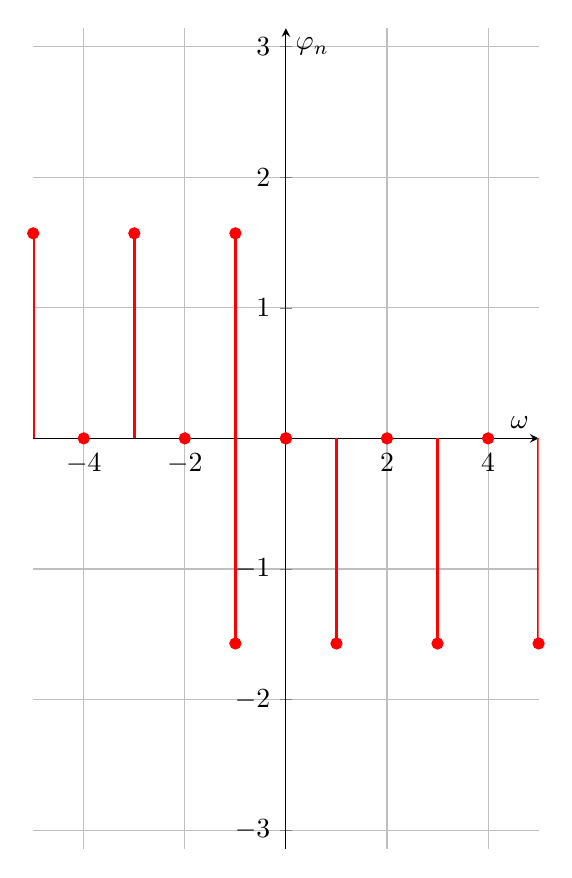
\begin{tikzpicture}
	\begin{axis}[axis lines=middle, grid=both, height=12cm, width=8cm, xmin=-5, xmax=5, ymin=-pi, ymax=pi, xlabel = $\omega$, ylabel = $\varphi_n$]
		\foreach \x in {0,...,5}{
			\addplot[mark=none, red, very thick] coordinates { ({\x * 2 - 1}, 0) ({\x * 2 - 1}, {-pi/2}) };
			\addplot[mark=none, red, very thick] coordinates { ({-\x * 2 - 1}, 0) ({-\x * 2 - 1}, {pi/2}) };
			\addplot[only marks, red] coordinates{ ({\x * 2 - 1}, {-pi/2}) };
			\addplot[only marks, red] coordinates{ ({\x * 2}, {0}) };
			\addplot[only marks, red] coordinates{ ({-\x * 2 - 1}, {pi/2}) };
			\addplot[only marks, red] coordinates{ ({-\x * 2}, {0}) };
		}
	\end{axis}
\end{tikzpicture}}\\[3pt]
				\hline
			\end{tabular}
		\end{minipage}
		\begin{minipage}[]{0.5\textwidth}
			\textbf{Polarkoordinaten der komplexen Fourierkoeffizienten $c_k$ werden in zwei Diagrammen dargestellt:}\\[3pt]
			\fbox{Amplitude $= |c_k|$} \fbox{Phase $= \arg(c_k)$}\\[3pt]
			\scalebox{0.8}{
				\begin{tabular}{lllll}
					(I) & Amplituden & $\rightarrow$ & Achensymmetrisch & \fbox{$|c_n| = |c_{-n}|$}\\[6pt]
					(II) & Phasen & $\rightarrow$ & Punktsymmetrisch & \fbox{$\arg(c_n) = \arg(c_{-n})$}\\[3pt]
				\end{tabular}\\[6pt]
			}
			\textbf{Verknüpfung zum Einseitigen Amplituden-/Phasendiagramm: für $n \geq 0$ gilt:}\\[3pt]
			\fbox{$\varphi_n$ gleich wie (2)} \fbox{$\varphi_n = \arg(c_n)$}\\[3pt]
			\fbox{$|c_n| = \dfrac{1}{2} \cdot A_n$} \fbox{$A_0 = |\dfrac{a_0}{2}| = |c_0|$}\\[3pt]
			\textbf{Umrechnung von Sinus- und Kosinusdiagramm (1):}\\[3pt]
			\fbox{$c_n = \dfrac{a_n - \mathrm{j} b_n}{2}$} \fbox{$\varphi_n = \arg(a_n - \mathrm{j} b_n)$}
		\end{minipage}

	\subsection{Spezialfälle (zu den Phasendiagrammen: 1, 2, 3)}
		\begin{tabular}{ll}
			Funktion $f$ gerade & (1) Sinusphasendiagramm überall $0$\\[3pt]
			 & (2, 3) Phasendiagramm enthält nur die Werte $0$ und $\pi$\\[3pt]
	 		Funktion $f$ ungerade & (1) Kosinusphasendiagramm überall $0$\\[3pt]
	 		 & (2, 3) Phasendiagramm enthält nur die Werte $\pm \dfrac{\pi}{2}$\\[3pt] 
	 		 & (oder $0$ falls Amplitudenwert $= 0$)\\[3pt]
	 		Ähnlichkeit $g(t) = f(r \cdot t)$ & (1, 2, 3) Das Spektrum von $g$ ist das horizontal mit dem Faktor $r$\\[3pt]
	 		 & gestrecktes Spektrum vom $f$\\[3pt]
	 		Zeitverschiebung $g(t) = f(t + t_0)$ & (1) (siehe auch 3.4.4, Zeitverschiebung (S. 4))\\[3pt]
	 		 & (2, 3) Amplitudendiagramme sind identisch.\\[3pt]
	 		 & (2, 3) Phasendiagramme: Die Säule der Frequenz $k \omega_0$ wächst um $k \omega_0 t_0$\\[3pt]
	 		Weisses Rauschen & Überlagerung von Schwingungen aller möglichen Frequenzen\\[3pt]
	 		 & mit gleichen Amplituden und zufälligen Phasen.\\[3pt]
		\end{tabular}

	\subsection{Zeitbereich und Frequenzbereich}
		\begin{minipage}[]{0.5\textwidth}
			\centering
			\scalebox{1.6}{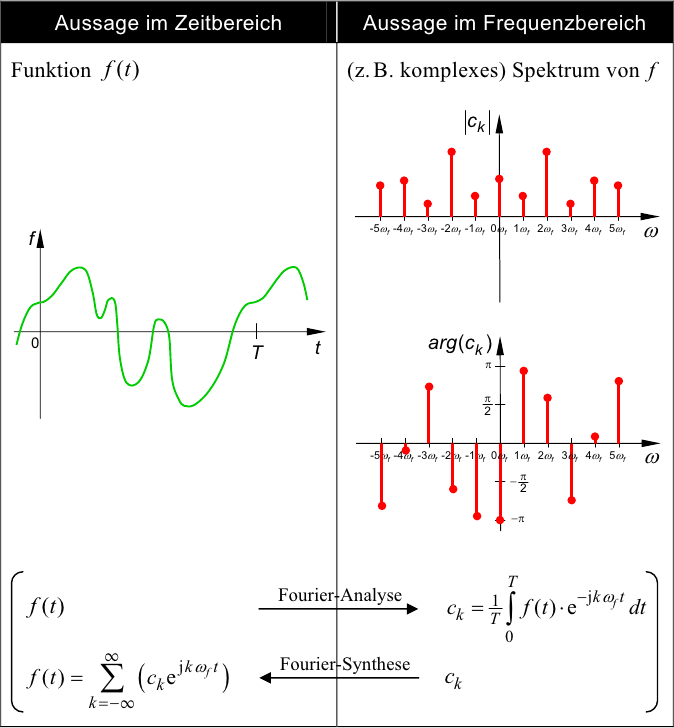
\includegraphics[width=0.5\textwidth]{pics/Spektren/ZeitUndFrequenzbereich1.png}}
			\captionof{figure}{Quelle: Skript KomFour}
			\centering
			\scalebox{1.6}{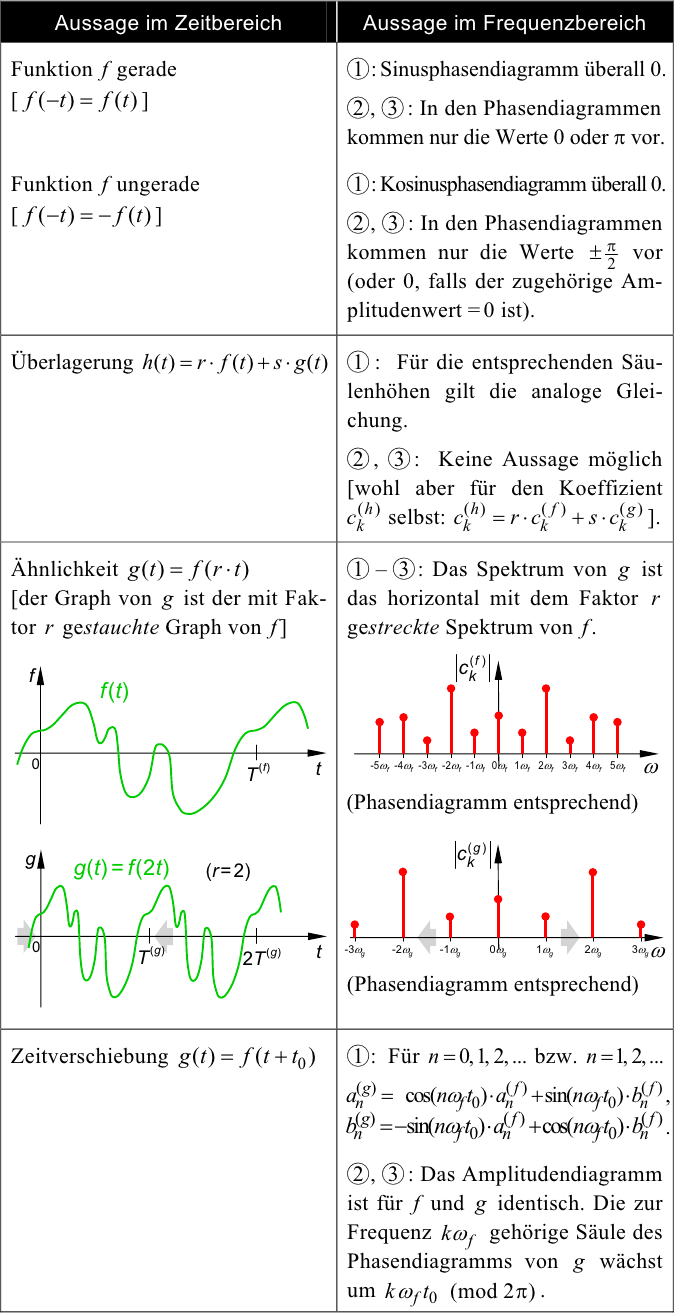
\includegraphics[width=0.5\textwidth]{pics/Spektren/ZeitUndFrequenzbereich2.png}}
			\captionof{figure}{Quelle: Skript KomFour}
		\end{minipage}
		\begin{minipage}[]{0.5\textwidth}
			\centering
			\scalebox{1.6}{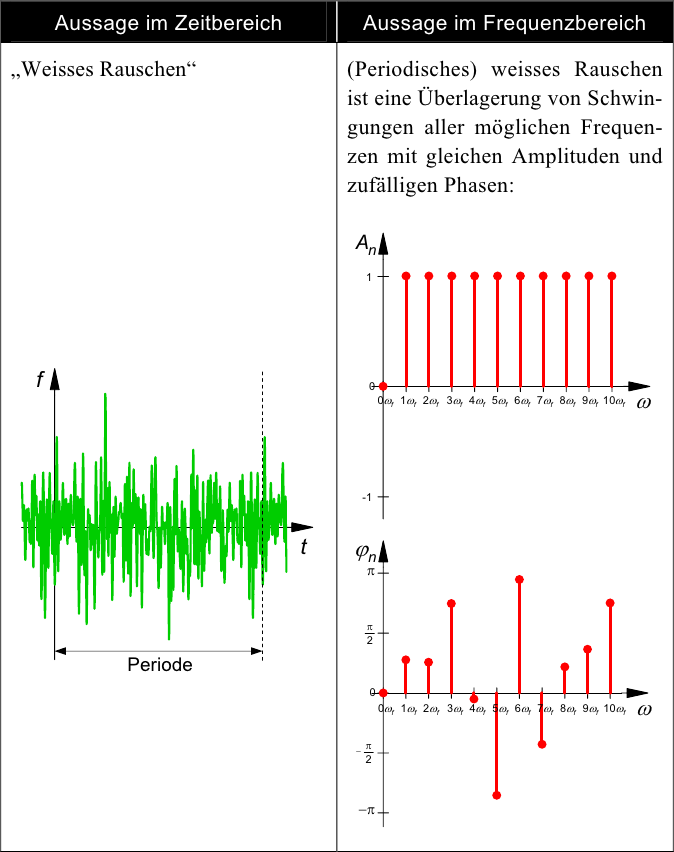
\includegraphics[width=0.5\textwidth]{pics/Spektren/ZeitUndFrequenzbereich3.png}}
			\scalebox{1.6}{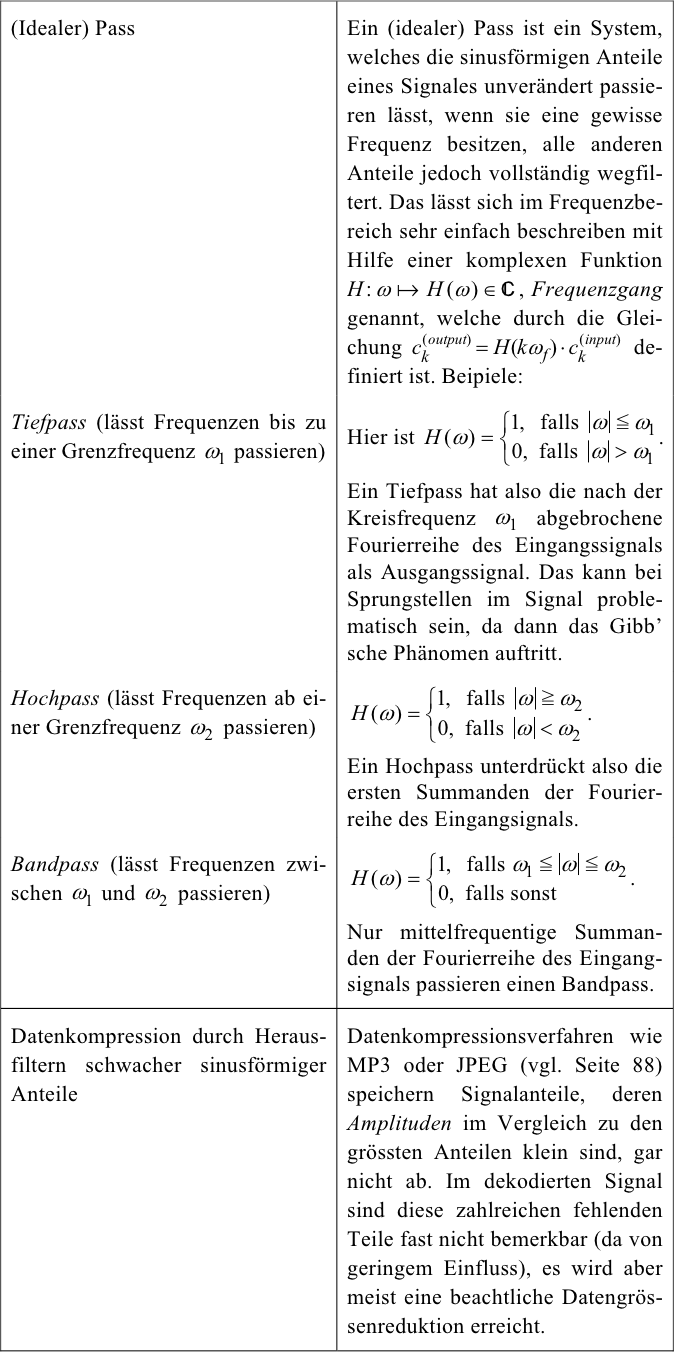
\includegraphics[width=0.5\textwidth]{pics/Spektren/ZeitUndFrequenzbereich4.png}}
			\captionof{figure}{Quelle: Skript KomFour}
		\end{minipage}

		